\documentclass[handout, 10pt]{beamer}

%\usepackage[backend=bibtex,firstinits=true,style=verbose-inote,citestyle=authortitle]{biblatex}
\usepackage{bm}
\usepackage{graphicx}
\usepackage{subcaption}
\usepackage{amsmath}
\usepackage{amsfonts}
\usepackage{makecell}
\usepackage{filecontents}
\usepackage{biblatex}
\usepackage{xcolor}
\usepackage{subcaption}
% \newcommand{\expect}[2][]{
\ifthenelse{\equal{#1}{}}{
\mathbb{E}\left[#2\right]
}{
\underset{#1}{\mathbb{E}}\left[#2\right]
}}

\newcommand{\cov}[2][]{
\ifthenelse{\equal{#1}{}}{
\text{Cov}\left[#2\right]
}{
\underset{#1}{\text{Cov}}\left[#2\right]
}}


\newcommand{\var}[2][]{
\ifthenelse{\equal{#1}{}}{
\text{Var}[#2]
}{
\underset{#1}{\text{Var}}[#2]
}}

\newcommand{\loss}[2][]{
\ifthenelse{\equal{#1}{}}{
\mathcal{L}(#2)
}{
\mathcal{L}_{#1}(#2)
}}

\newcommand{\kl}[2]{
\text{D}_\text{KL}[#1 \parallel #2]
}

\newcommand{\R}{\mathbb{R}}
%\newcommand{\Prob}{\mathbb{P}}

\newcommand{\1}[1]{\mathds{1}\{#1\}}


%\usecolortheme{dolphin}
\setbeamertemplate{navigation symbols}{}
\setbeamertemplate{section in toc}{\inserttocsectionnumber.~\inserttocsection}

\begin{filecontents*}{references.bib}
@inproceedings{IMNET,
  title={Learning implicit fields for generative shape modeling},
  author={Chen, Zhiqin and Zhang, Hao},
  booktitle={Proceedings of the IEEE Conference on Computer Vision and Pattern Recognition},
  pages={5939--5948},
  year={2019}
}
\end{filecontents*}

\addbibresource{references.bib}


\title{Learning implicit fields for generative shape modeling\footnote{\citepaper{IMNET}}}
%\subtitle{}
%\author{Ivan Skorokhodov}
%\date{}
%\logo{
\includegraphics[height=1cm]{images/ipavlov-logo.png}}

\newcommand{\citepaper}[1]{\citetitle{#1} by \citeauthor{#1}, \citeyear{#1}}

%\graphicspath{{./images}}

%\usetheme{lucid}
\begin{document}

\begin{frame}
    \titlepage
\end{frame}

\begin{frame}{Overview}
\begin{itemize}
    \item\pause There are different ways to represent 3D shapes: voxel grids, octrees, point clouds, etc.
    \item\pause It is quite expensive (in terms of GPU memory) to train a decoder for such kind of outputs
    \item\pause So authors employed an INR-like decoder to output 3D shapes
    \item\pause They test the approach on several tasks:
    \begin{itemize}
        \item\pause Auto-encoding
        \item\pause 3D-shape generation
        \item\pause 2D-shape generation (generating MNIST digits)
    \end{itemize}
    \item\pause They obtain strong results, but the model is slower to train and run
\end{itemize}
\end{frame}

\begin{frame}{Implicit Field Decoder}
Authors propose \textit{IM-NET}: an INR-like decoder
\begin{figure}
    \centering
    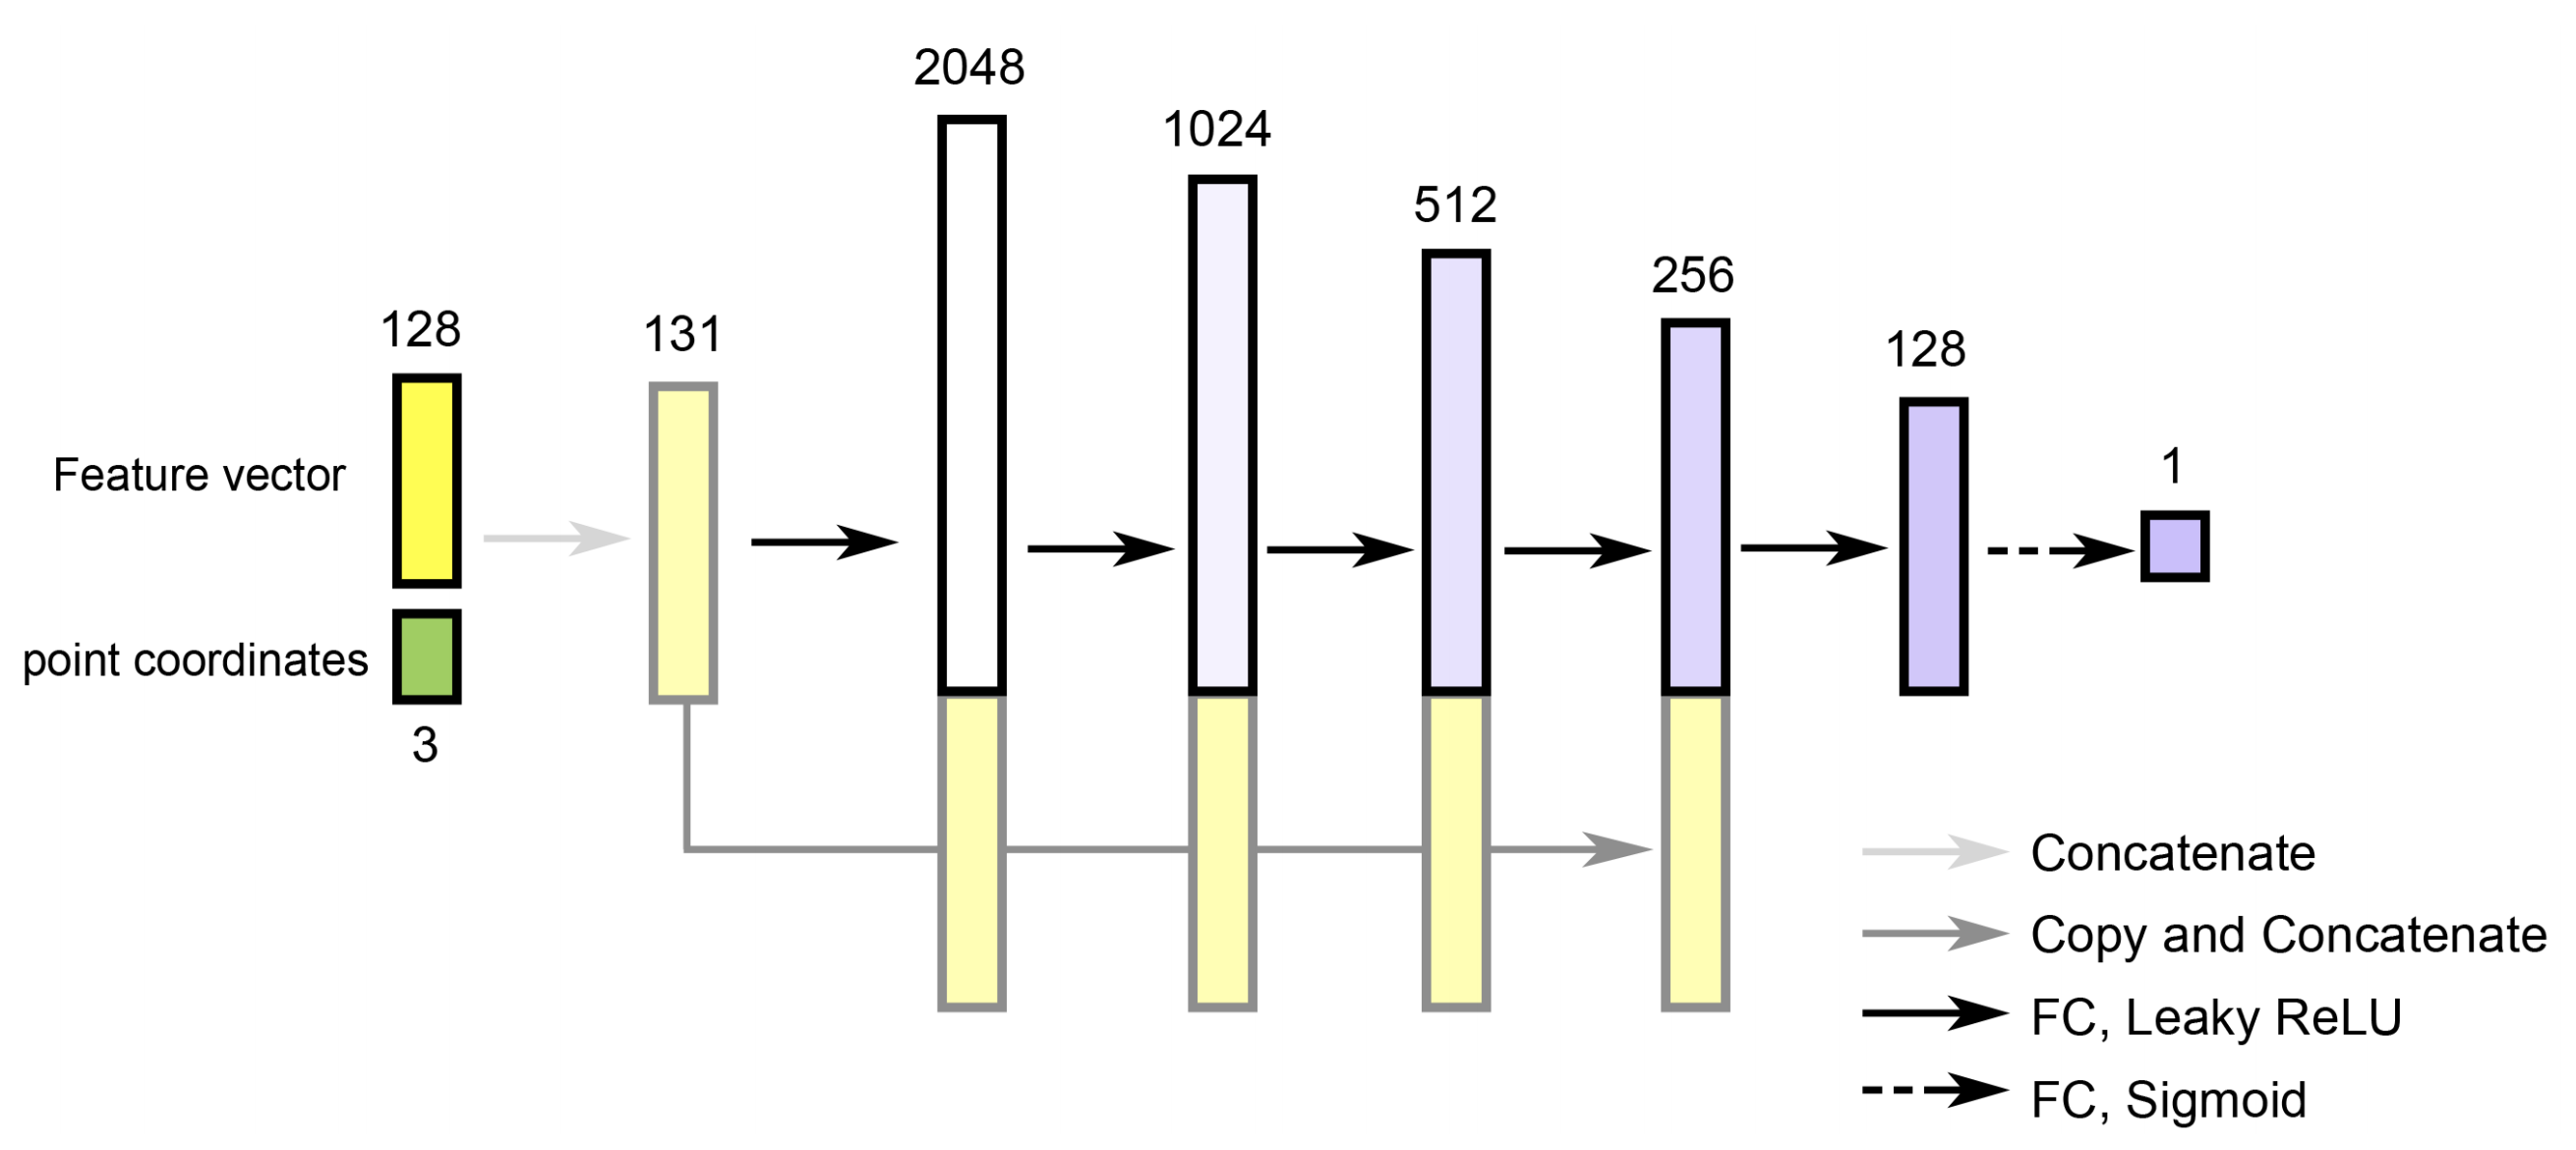
\includegraphics[width=0.8\textwidth]{images/im-net}
\end{figure}
\begin{itemize}
    \item\pause This decoder:
    \begin{itemize}
        \item\pause takes a coordinate $(x,y,z)$ and an image embedding
        \item\pause outputs 1 or 0, denoting if a point is a part of the shape or not
    \end{itemize}
    \item\pause They train it with the MSE loss
\end{itemize}
\end{frame}


\begin{frame}{Data preparation}
Authors perform the following data preparation steps:
    \begin{itemize}
        \item\pause Downsample training examples to different resolutions: $16^3, 32^3, 64^3, 128^3$.
        \item\pause Sample points near closer to a surface with higher probability
    \end{itemize}
    \begin{figure}
        \begin{subfigure}{.45\textwidth}
            \centering
            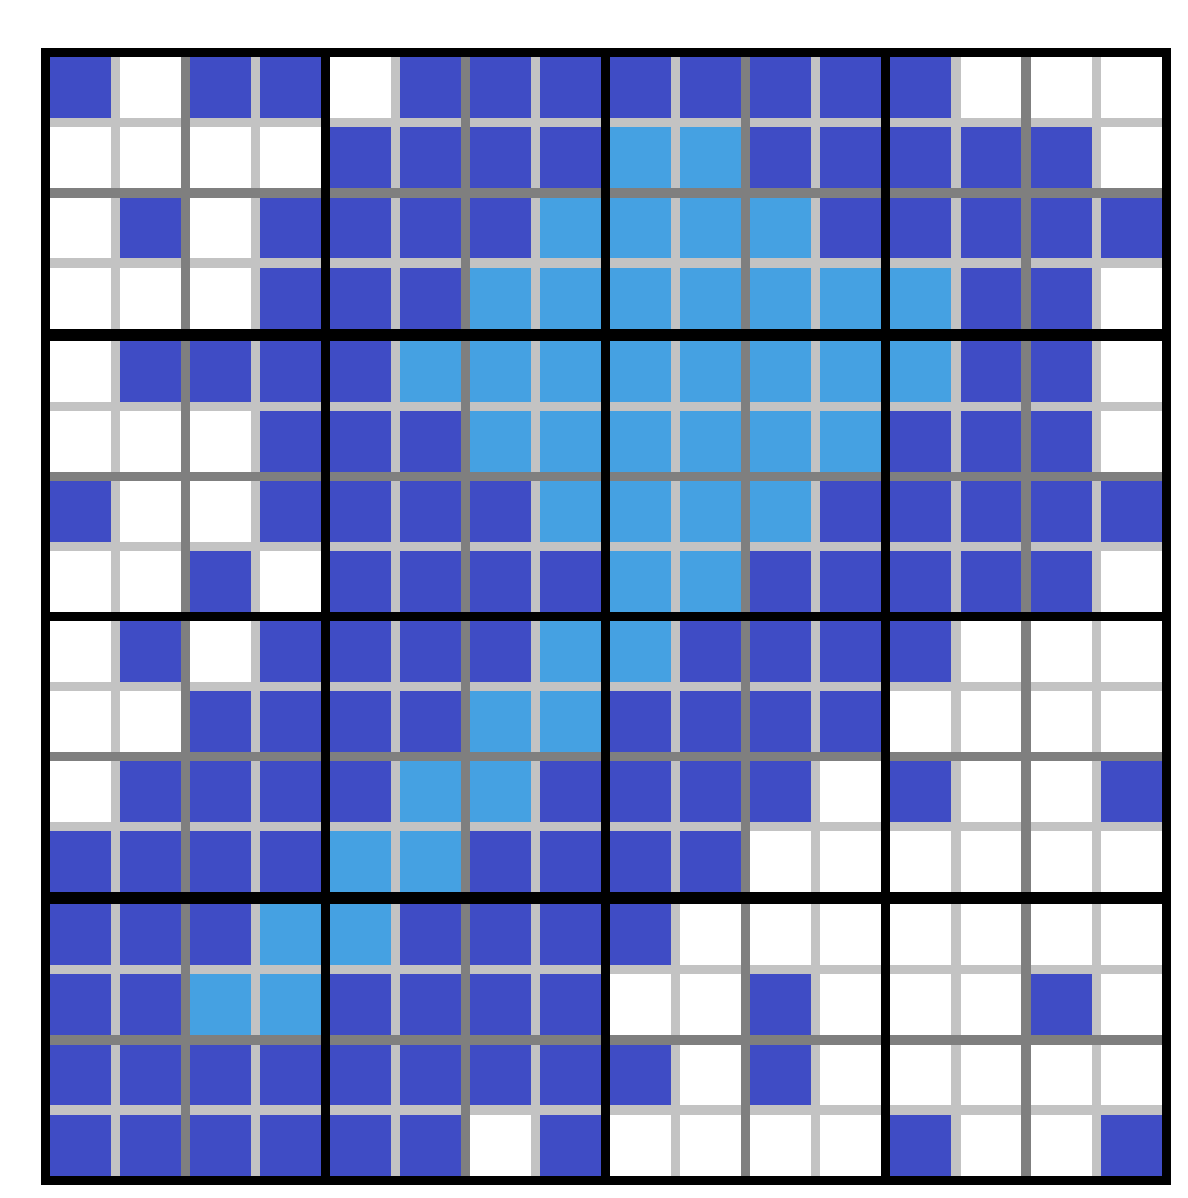
\includegraphics[width=0.9\textwidth]{images/sampling-strategy-1}
            \caption{Main strategy: sample points 2 voxels away from the surface}
        \end{subfigure}
        \begin{subfigure}{.45\textwidth}
            \centering
            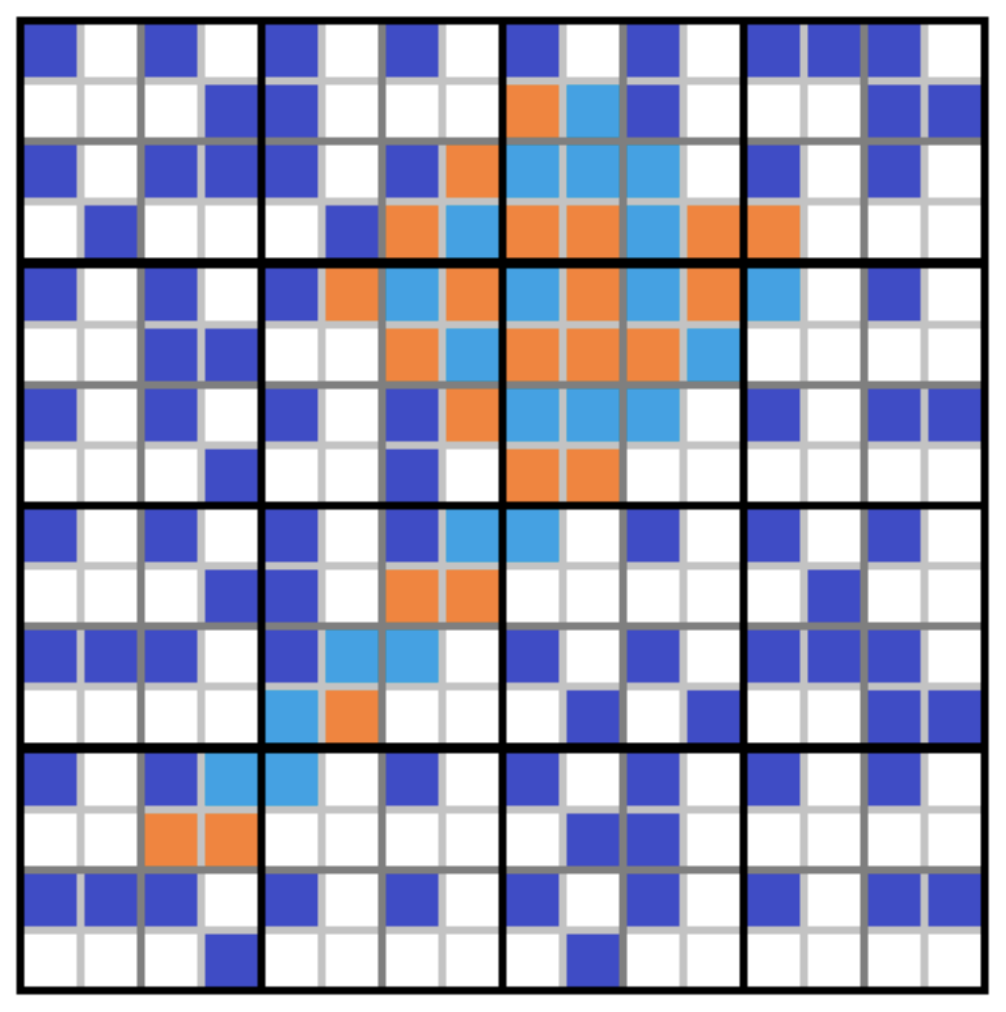
\includegraphics[width=0.9\textwidth]{images/sampling-strategy-2}
            \caption{Auxiliary strategy: sample points evenly with a stride}
        \end{subfigure}
    \end{figure}
\end{frame}


\begin{frame}{3D-shape auto-encoding}
    \begin{itemize}
        \item\pause Use a CNN-encoder (with conv3d layers) as Encoder
        \item\pause Use a IM-NET as Decoder
        \item\pause They use a CNN-decoder as a baseline decoder
    \end{itemize}
\end{frame}


\begin{frame}{3D-shape auto-encoding samples}
\begin{figure}
    \centering
    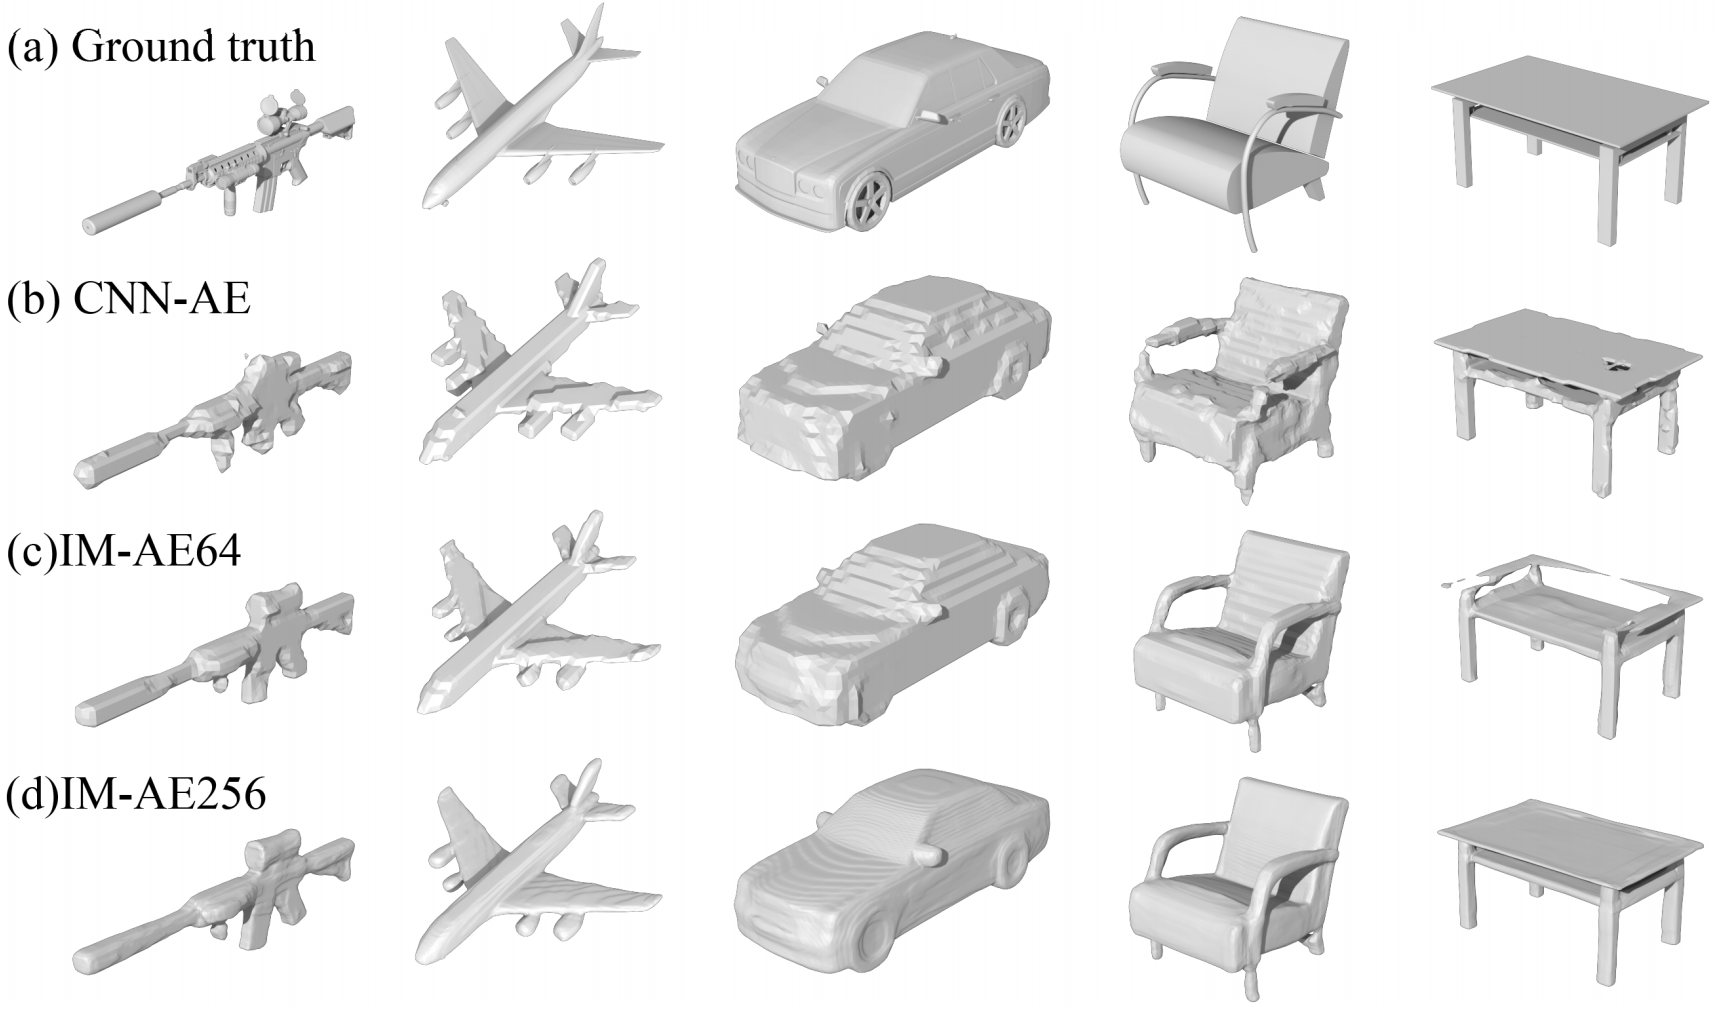
\includegraphics[width=0.8\textwidth]{images/3d-shape-autoencoding-samples}
\end{figure}
\end{frame}


\begin{frame}{3D-shape auto-encoding results}
\begin{figure}
    \centering
    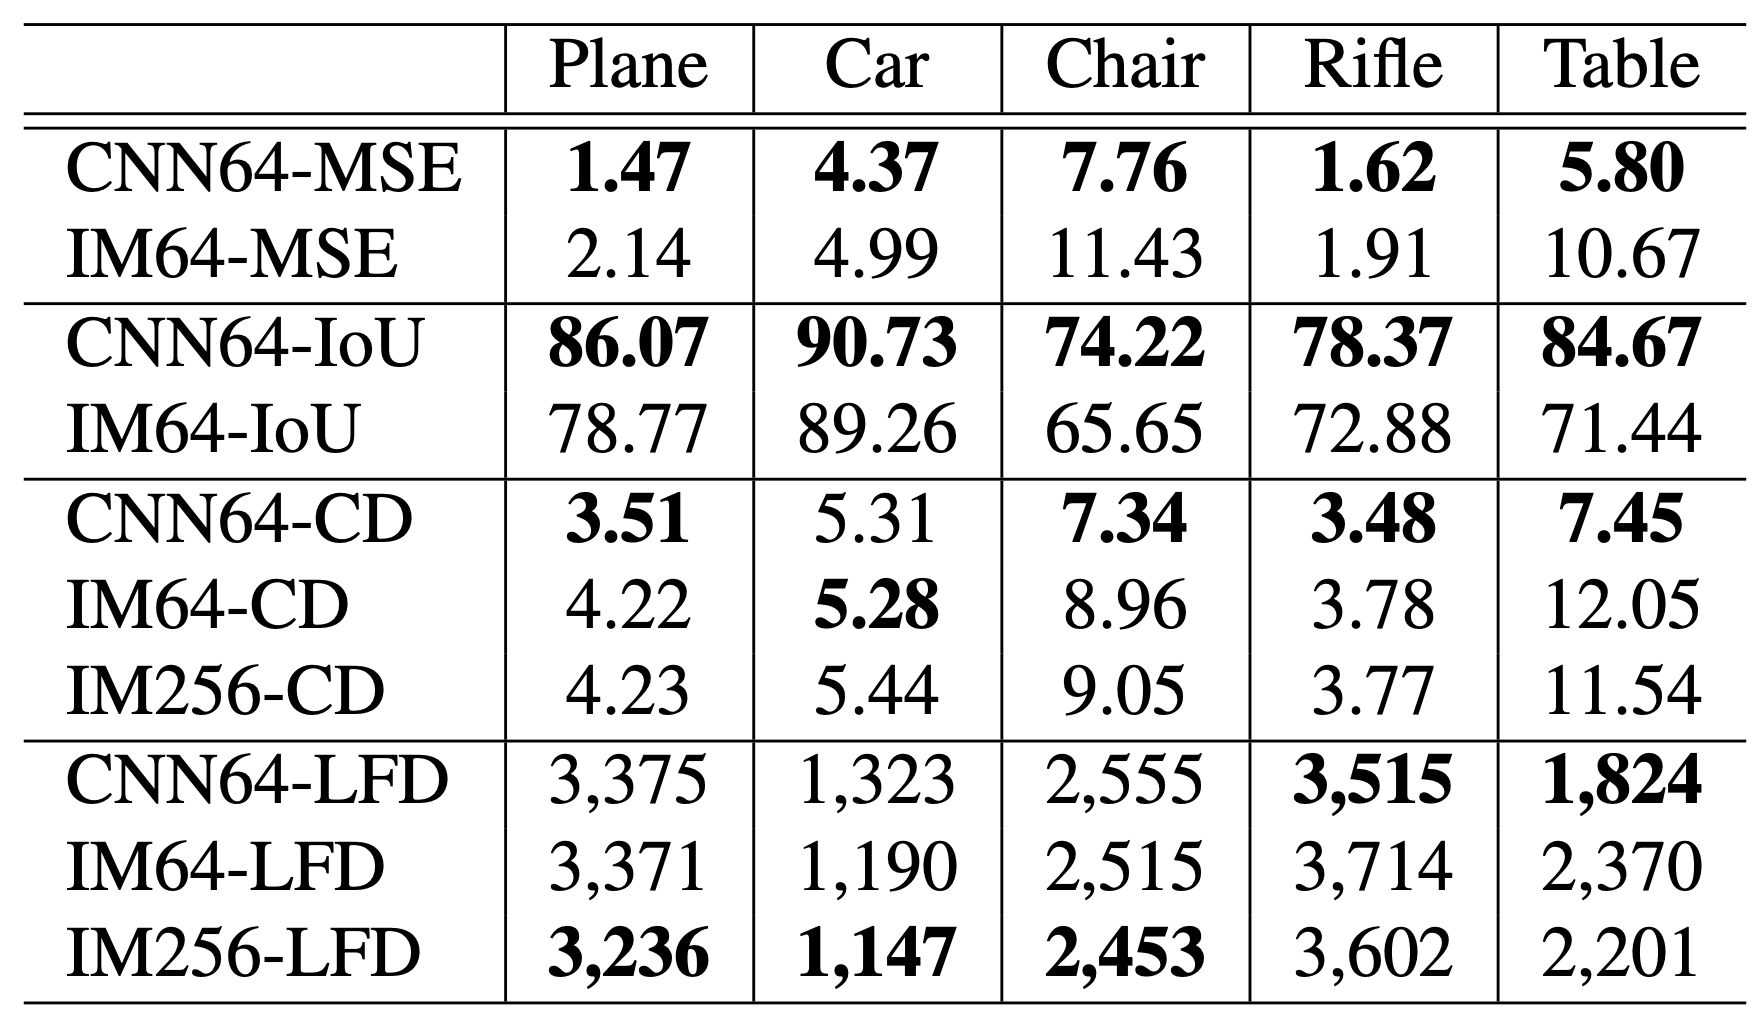
\includegraphics[width=0.5\textwidth]{images/3d-shape-autoencoding-results}
\end{figure}
\begin{itemize}
    \item\pause IM-NET works worse on all the metrics except LFD
    \item\pause But visually its samples are better
    \item\pause Authors claim that all the metrics except LFD are bad (and provide some argumentation for this)
    \item\pause LFD (Light Field Descriptor) is computed by taking several 2D renderings of two shapes from different angles and comparing the results
\end{itemize}
\end{frame}


\begin{frame}{3D-shape generation}
    \begin{figure}
        \centering
        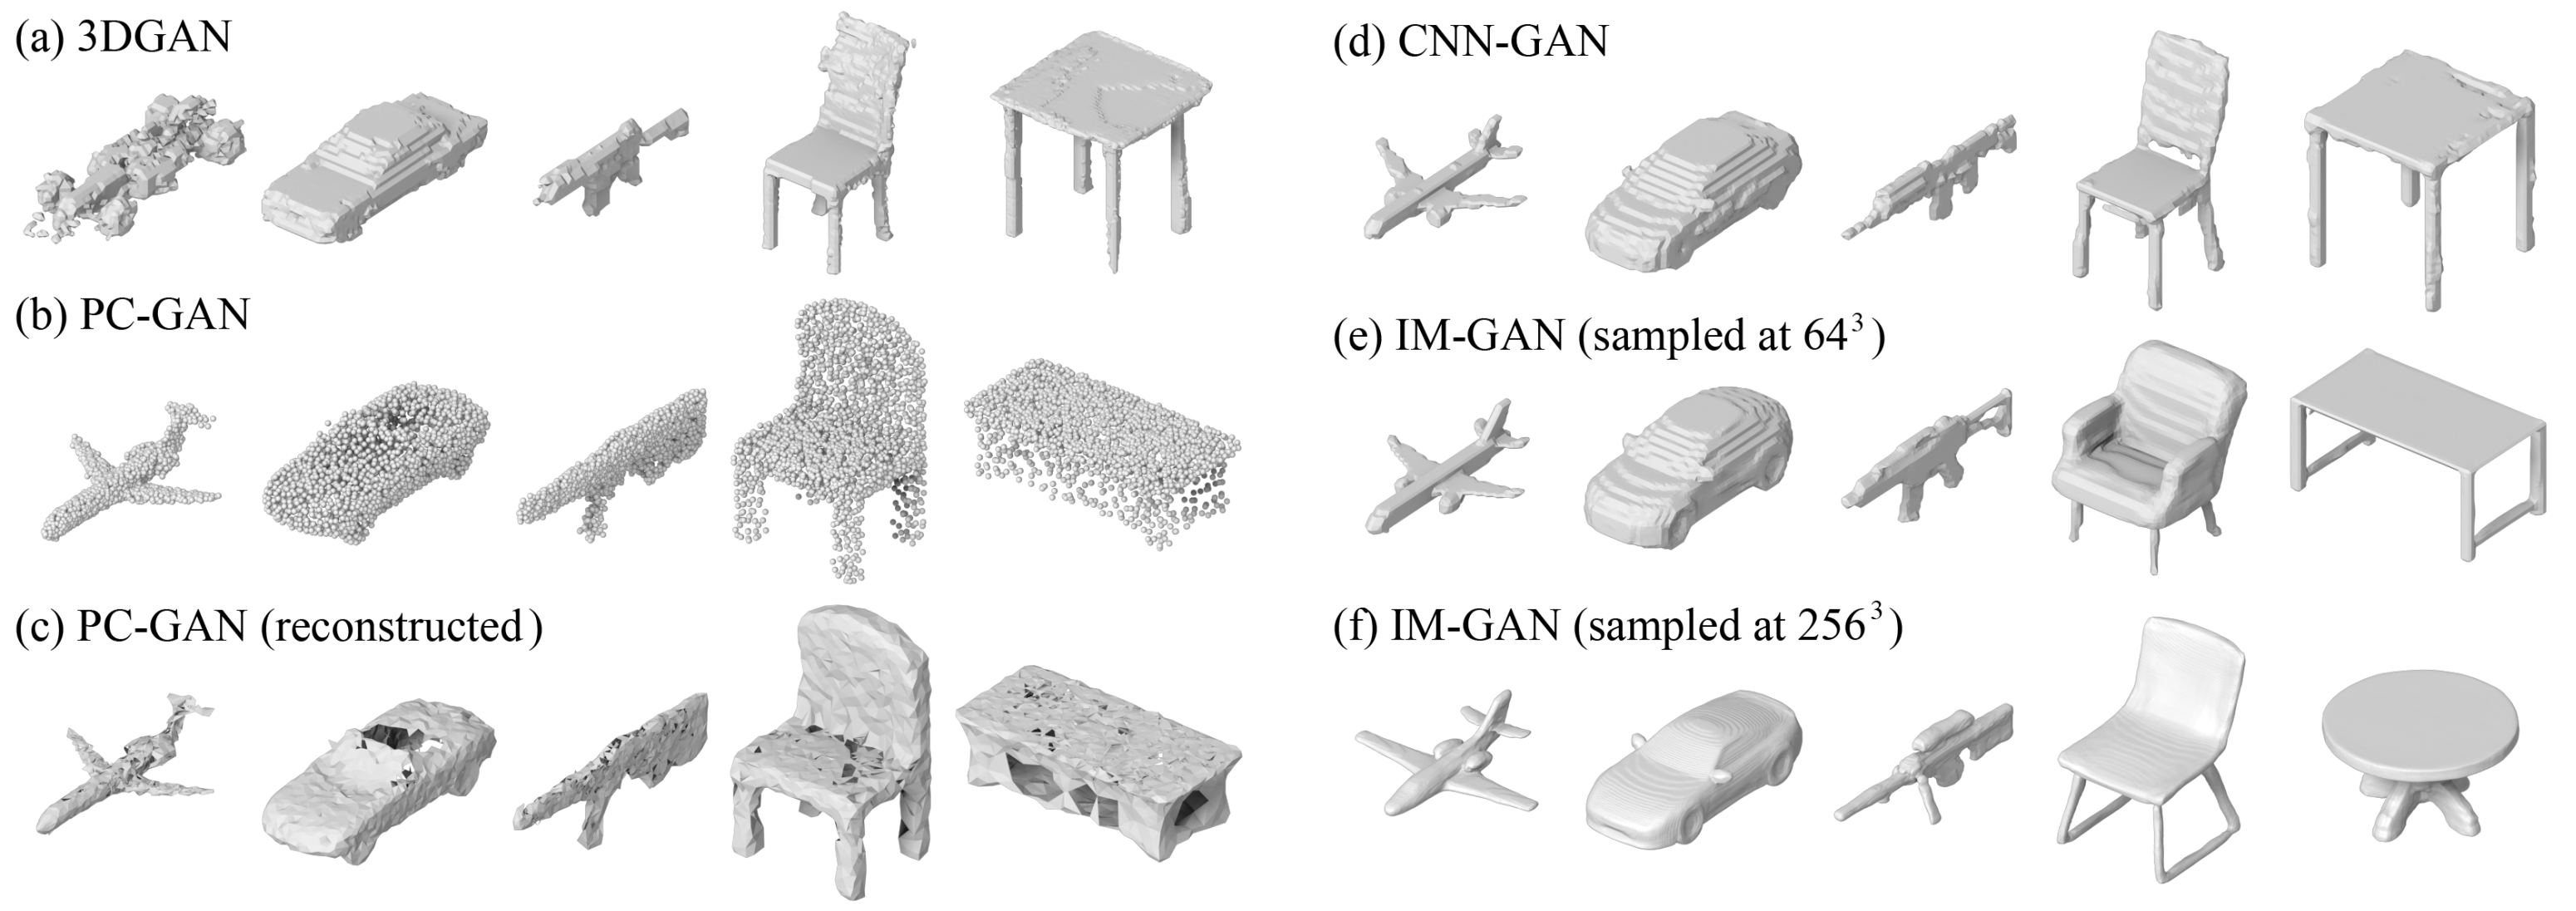
\includegraphics[width=\textwidth]{images/3d-generation-samples}
        \caption{Authors trained a GAN model on latent codes of the autoencoder and used IM-NET or CNN Decoder to decode the generated codes}
    \end{figure}
\end{frame}


\begin{frame}{3D-shape interpolation}
    \begin{figure}
        \centering
        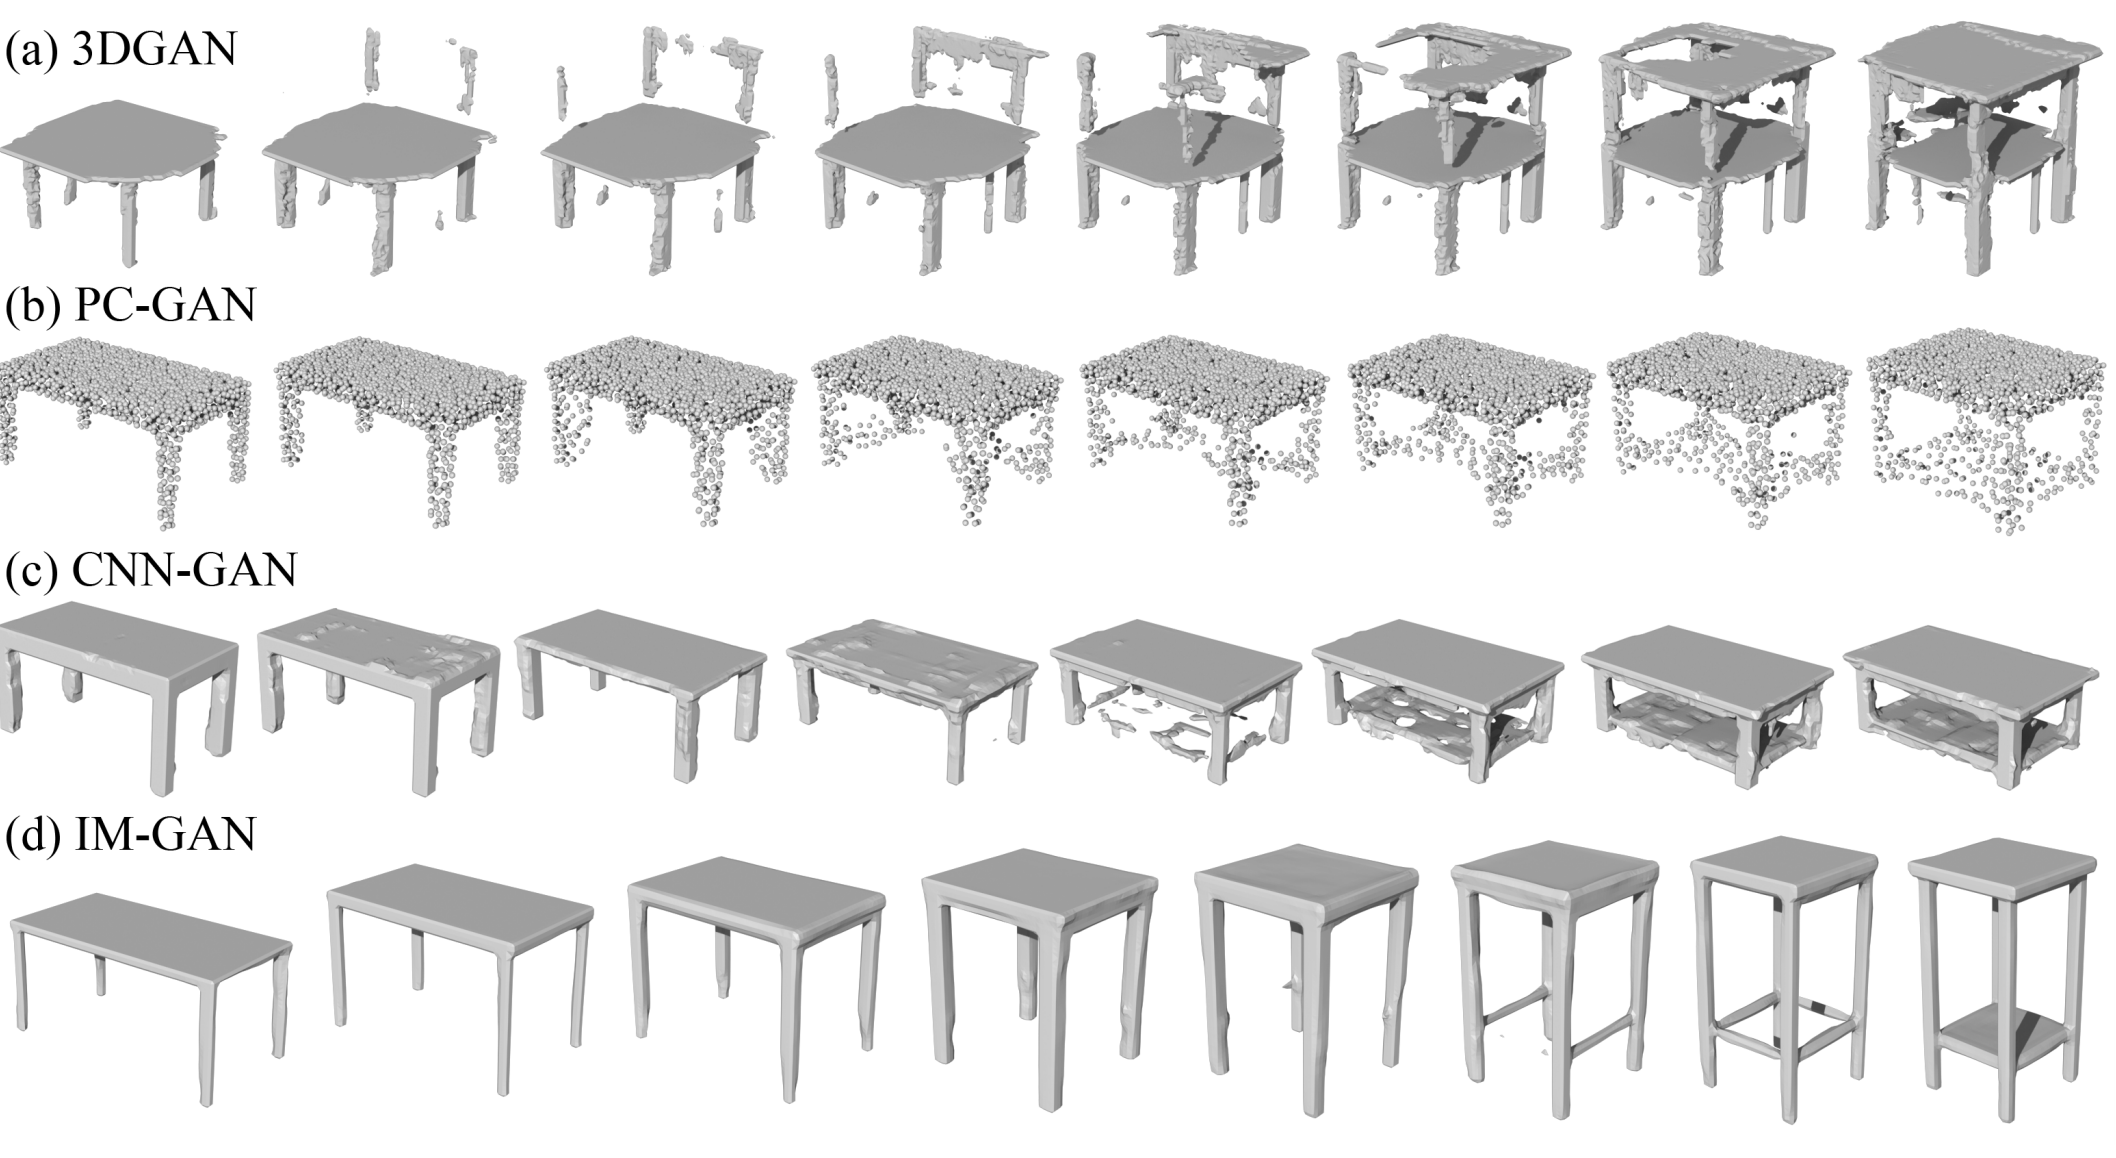
\includegraphics[width=\textwidth]{images/3d-generation-interpolation-samples}
    \end{figure}
\end{frame}


\begin{frame}{2D-shape generation}
2D shape generation models:
\begin{itemize}
    \item\pause Train a GAN model on latent codes of the autoencoder and use IM-NET or CNN decoder
    \item\pause Train VAE/WGAN/DCGAN
    \item\pause Train VAE/WGAN but use IM-NET Decoder instead of decoder/generator part
\end{itemize}
\pause

For 2D-shape generation, they train all the models on only 5000 images.
    \begin{figure}
        \centering
        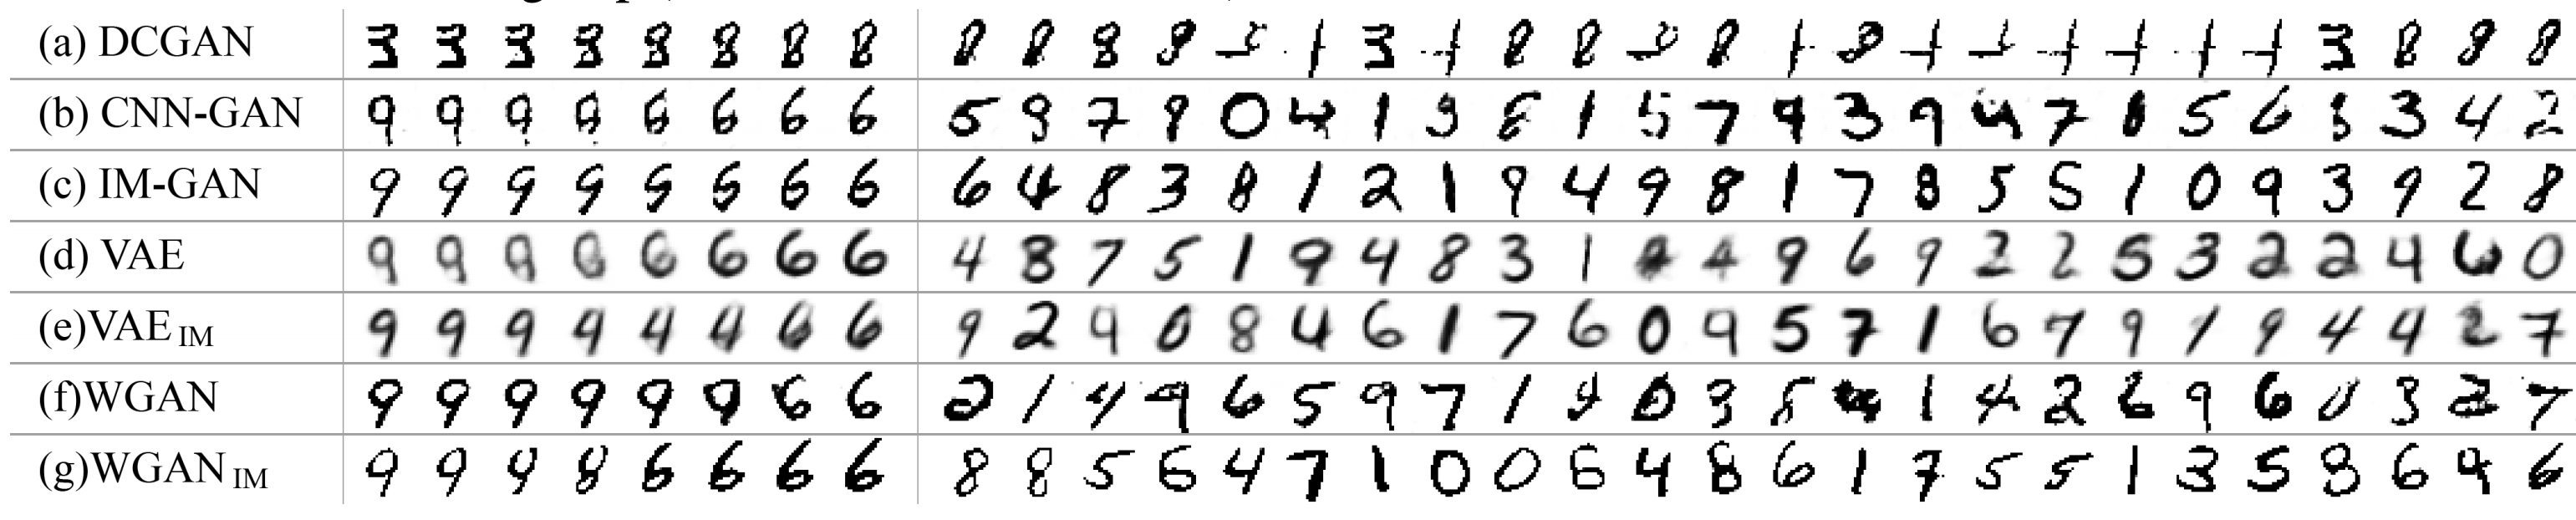
\includegraphics[width=\textwidth]{images/2d-generation-samples}
    \end{figure}
\end{frame}


\begin{frame}{Conclusion}
Pros
\begin{itemize}
    \item\pause Smoother surfaces compared to voxel grids
    \item\pause An ability to learn a complete shape (no need in parts annotation)
    \item\pause Super-resolution and progressive growing without architectural changes
    \item\pause Traditional CNN decoders are limited by GPU memory size (we cannot output high resolutions) during training, while INRs are not (since we can compute values only in points of interest)
\end{itemize}

Cons
\begin{itemize}
    \item\pause Much longer training time (up to $30\times$)
    \item\pause Authors didn't test the approach on more complex datasets
    \item\pause We need to train 1 model per category (likely because of weights sharing in Decoder)
\end{itemize}
\end{frame}


\end{document}
